\section{Introduction}
In this report we are going to have a look in depth about the Knowledge Distillation. Some papers were written about that, in particular, the idea was to have a student who distills knowledge from the teacher and who has comparable reliability but higher speed, so that, unlike the latter can be used in a production environment.\\
In the paper\cite{ban} that we are going to deepen, a further step is taken, the distillation of knowledge is done by a student of same complexity to that of the teacher. The authors in this case observe an improvement in the performance of the student networks, and surprisingly the improvement also occurs with subsequent generations of students. In the paper the new networks are called Born Again Networks.
My work will be to replicate those results in a practical way with real datasets, trying to explain as best as possible every step, making available all the code produced during my experiments. I'll also try to 
experiment some variant just to annotate what are the changes.\\
In the introduction I will just prepare the environment that will be used for the next experiments, while in the following parts of the report I will implement the algorithm and then perform all the tests.

\subsection{Residual Network}
One of the models used in the reference paper Wide Residual Network, presented in another paper indicated in the bibliography\cite{wresnet}. In essence, the creators of the new model (WRNs) suggest that a less "deep" structure can minimize the problem of diminishing feature reuse so that even a fraction of improvement needs to double the layers. Until now, neural networks were made deeper and deeper to reduce the number of parameters, but the authors of the paper found that compared to deep resnet presented here \cite{deepresnet} they needed 50 times less layers.\\
They claim that a WResNet with 16 layers has an accuracy comparable to a DResNet with 1000 layers, and is also faster in training.\\
Looking at the code provided by the authors, there is only one implementation with the pytorch framework, but the intention is to complete the task with 
Tensorflow 2.0, so it is interesting to have a version of it also for the framework I used in this work.
\newpage
The first step will be the coding of the model, which I think it may be interesting to develop also using the Tensorflow Subclassing API in order to have a clean and usable version later, even at the cost of meeting some problems that will be mentioned later.\\
From the paper\cite{wresnet} we can see the different kind of blocks\\

\begin{figure}[h!]
\centering
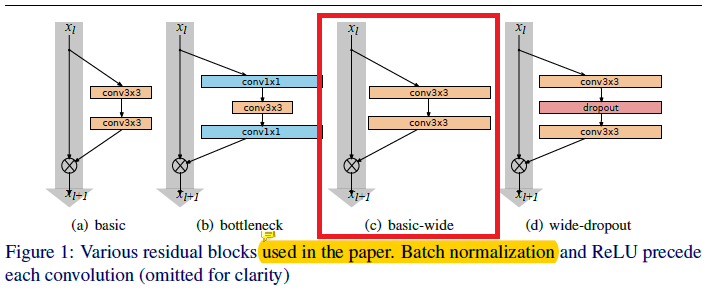
\includegraphics[width=0.8\textwidth]{wresnet.png}
\end{figure}

Let's see the code of the Residual Layer
\lstset{language=Python}
\lstset{frame=lines}
\lstset{caption={The code of the Residual Layer}}
\lstset{label={lst:code_direct}}
\lstset{basicstyle=\footnotesize}
\begin{lstlisting}
class ResidualBlock(layers.Layer):
  def __init__(self, filters, kernel_size, dropout,
               dropout_percentage, strides=1, **kwargs):
    super(ResidualBlock, self).__init__(**kwargs)
    self.conv_1 = layers.Conv2D(filters, (1, 1), strides=strides)
    self.bn_1 = layers.BatchNormalization()
    self.rel_1 = layers.ReLU()
    self.conv_2 = layers.Conv2D(filters, kernel_size, padding="same",
                                strides=strides)
    self.dropout_layer = layers.Dropout(dropout_percentage)
    self.bn_2 = layers.BatchNormalization()
    self.rel_2 = layers.ReLU()
    self.conv_3 = layers.Conv2D(filters, kernel_size, padding="same")
    self.add = layers.Add()
    self.dropout = dropout
    self.strides = strides


  def call(self, inputs, training=None):
    x = inputs
    if self.strides > 1:
      x = self.conv_1(x)
    res_x = self.bn_1(inputs)
    res_x = self.rel_1(res_x)
    res_x = self.conv_2(res_x)
    if self.dropout:
      res_x = self.dropout_layer(res_x, training=training)
    res_x = self.bn_2(res_x)
    res_x = self.rel_2(res_x)
    res_x = self.conv_3(res_x)
    inputs = self.add([x, res_x])
    return inputs
 
\end{lstlisting}
The block is the one shown in the figure, with a parameter to activate the Dropout. The get\_config method instead is simply used to allow the user to save the model.
In the paper there is also the "bottleneck layer" that is neglected, and I will do the same in my work, focusing on the "basic" type.\\
The model instead is an aggregation of ResidualLayers that takes in input 2 parameters: k and d (d in the paper is called "l") , which are respectively the widening factor and the deepening factor.\\
Let's see the code of the Model:
\lstset{language=Python}
\lstset{frame=lines}
\lstset{caption={The code of the Wide Residual Network}}
\lstset{label={lst:code_direct}}
\lstset{basicstyle=\footnotesize}
\begin{lstlisting}
class WideResidualNetwork(models.Model):
  def __init__(self, n_classes, d, k, kernel_size=(3, 3),
               dropout=False, dropout_percentage=0.3, strides=1, includeTop=True, **kwargs):
    super(WideResidualNetwork, self).__init__(**kwargs)
    if (d-4)%6 != 0:
      raise ValueError('Please choose a correct depth!')
    
    self.dropout = dropout
    self.dropout_percentage = dropout_percentage
    self.N = int((d - 4) / 6)
    self.k = k
    self.d = d
    self.includeTop = includeTop
    self.kernel_size = kernel_size

    self.bn_1 = layers.BatchNormalization()
    self.rel_1 = layers.ReLU()
    self.conv_1 = layers.Conv2D(16, (3, 3), padding='same')
    self.conv_2 = layers.Conv2D(16*k, (1, 1))
    self.dense = layers.Dense(n_classes)

    self.res_block_1 = [ResidualBlock(16*self.k, self.kernel_size, self.dropout,
     self.dropout_percentage) for _ in range(self.N)]
    self.res_single_1 = ResidualBlock(32*self.k, self.kernel_size, self.dropout,
     self.dropout_percentage, strides=2)
    self.res_block_2 = [ResidualBlock(32*self.k, self.kernel_size, self.dropout,
     self.dropout_percentage) for _ in range(self.N-1)]
    self.res_single_2 = ResidualBlock(64*self.k, self.kernel_size, self.dropout,
     self.dropout_percentage, strides=2)
    self.res_block_3 = [ResidualBlock(64*self.k, self.kernel_size, self.dropout,
     self.dropout_percentage) for _ in range(self.N-1)]
    self.pooling = layers.GlobalAveragePooling2D()
    self.activation_layer = layers.Activation("softmax")



  def call(self, inputs, training=None):
    x = self.bn_1(inputs)
    x = self.rel_1(x)
    x = self.conv_1(x)
    x = self.conv_2(x)
    for layer in self.res_block_1:
      x = layer(x, training=training)

    x = self.res_single_1(x, training=training)

    for layer in self.res_block_2:
      x  = layer(x, training=training)

    x = self.res_single_2(x, training=training)

    for layer in self.res_block_3:
      x = x = layer(x, training=training)

    x = self.pooling(x)
    x = self.dense(x)
    if self.includeTop:
        x = self.activation_layer(x)

    return x

\end{lstlisting}

In both cases I omitted the \textit{get\_config} function, as it is not useful for understanding the model.